\chapter{Simultaneous Localization and Learning: Optimizing Deep SE(3) Measurement Models}

\section{Motivation}

We present a novel way to use error-state Kalman filters to optimize deep probabilistic measurement models. Unlike traditional approaches that separate learning into two distinct training and evaluation phases, we instead use the modern tools of deep learning to embed a hyper-parametric model that can be optimized in tandem with trajectory estimates. Extending our prior work, we use matrix Lie groups to develop a parametrization with analytically differentiable loss functions and uncertainty propagation for 6 degree-of-freedom pose estimation. We show that by learning residuals to a predicted state, we can use the method of uncertainty injection onto the manifold to predict meaningful covariance estimates. As calibrated uncertainty estimates are crucial to reliable state estimation, we leverage ideas from the method of the statistical bootstrap to create a network we call a HydraNet that can produce covariance estimates that incorporate both epistemic and aleatoric uncertainty. Finally, we show how our system can be used to learn deep probabilistic measurement models in both two dimensions with planar Lidar data, and in three dimensions with stereo cameras.


\section{Global Lie Algebra Coordinates}

A basic composition in $\LieGroupSE{3}$ is given by,
\begin{align}
\Transform_c = \Transform_a \Transform_b.
\end{align}

We choose instead to use the composition in Lie algebra, or exponential coordinates, $\TransformVector = \MatLog{\Transform} = \Matlog{\Transform}$ (and similarly, $\Transform = \MatExp{\TransformVector} = \Matexp{\TransformVector}$), such that,

\begin{align}
\TransformVector_c = \matlogexpfn{\TransformVector_a}{\TransformVector_b} = \matlogexp{\TransformVector_a}{\TransformVector_b}.
\end{align}

This then allows us to derive the associated linear system in two ways.

Left perturbations:


\begin{align}
\delta \TransformVector_c =  \delta \TransformVector_a + \LieGroupAdjoint{\Transform_a} \delta \TransformVector_b.
\end{align}


Middle perturbations:

\begin{align}
\delta \TransformVector_c = \LeftJacobianSE(\TransformVector_c)^{-1} \LeftJacobianSE(\TransformVector_a) \delta \TransformVector_a + \LeftJacobianSE(\TransformVector_c)^{-1}  \LieGroupAdjoint{\Transform_a} \LeftJacobianSE(\TransformVector_b) \delta \TransformVector_b.
\end{align}

See the supplementary material for a derivation.


We can now define the loss function - negative log likelihood:

\begin{align}
\mathcal{L}(\TransformVector, \TransformVector_t, \Matrix{\Sigma}) = \Norm{\TransformVector \ominus \TransformVector_t}_{\Matrix{\Sigma}} + \log{|\Matrix{\Sigma}|}
\end{align}

where $\TransformVector_a \ominus \TransformVector_b = \matlogexpfn{\TransformVector_a}{-\TransformVector_b}$ 

\section{Experiments}

\begin{figure}
	\centering
	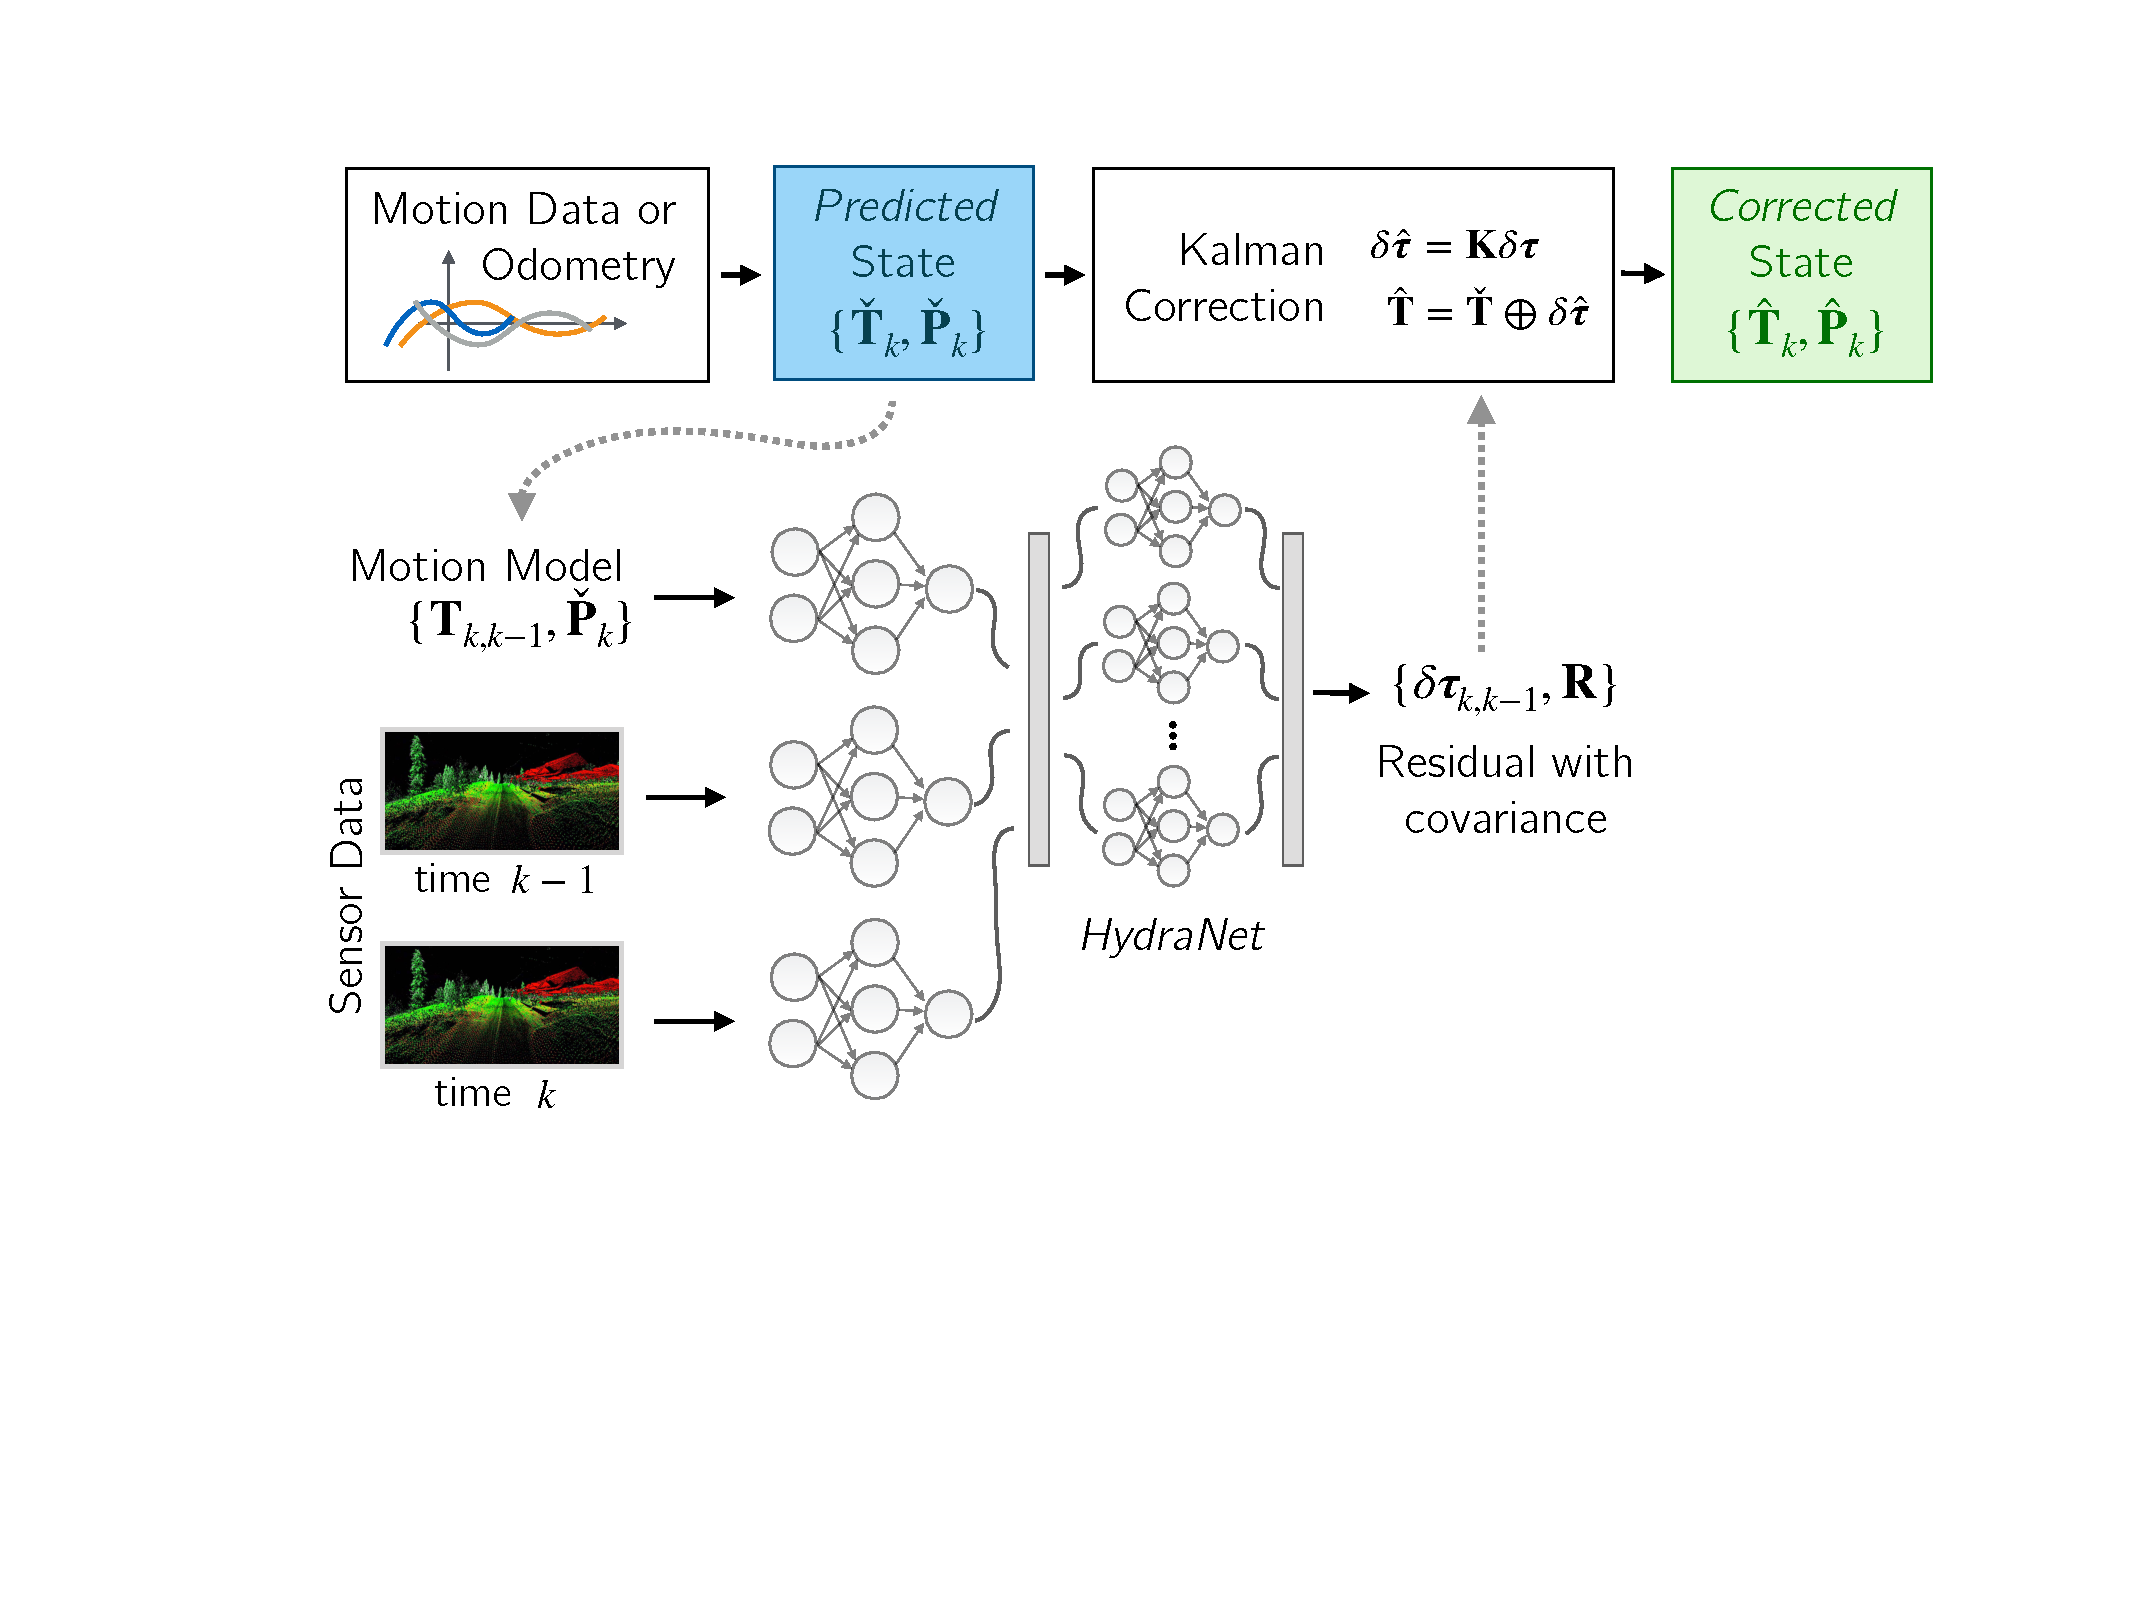
\includegraphics[width=0.9\textwidth]{lkf/rel_system}
	\caption{We present a novel way to train deep probabilistic measurement models with sparse ground truth data. Our architecture uses a multi-headed network we call a HydraNet to output residuals to a predicted state given sensor data and the state itself.}
	\label{fig:lkf_system}
\end{figure}


\section{Consistent Uncertainty Estimates}

\begin{figure}
    \centering
    \begin{subfigure}[]{0.9\textwidth}
    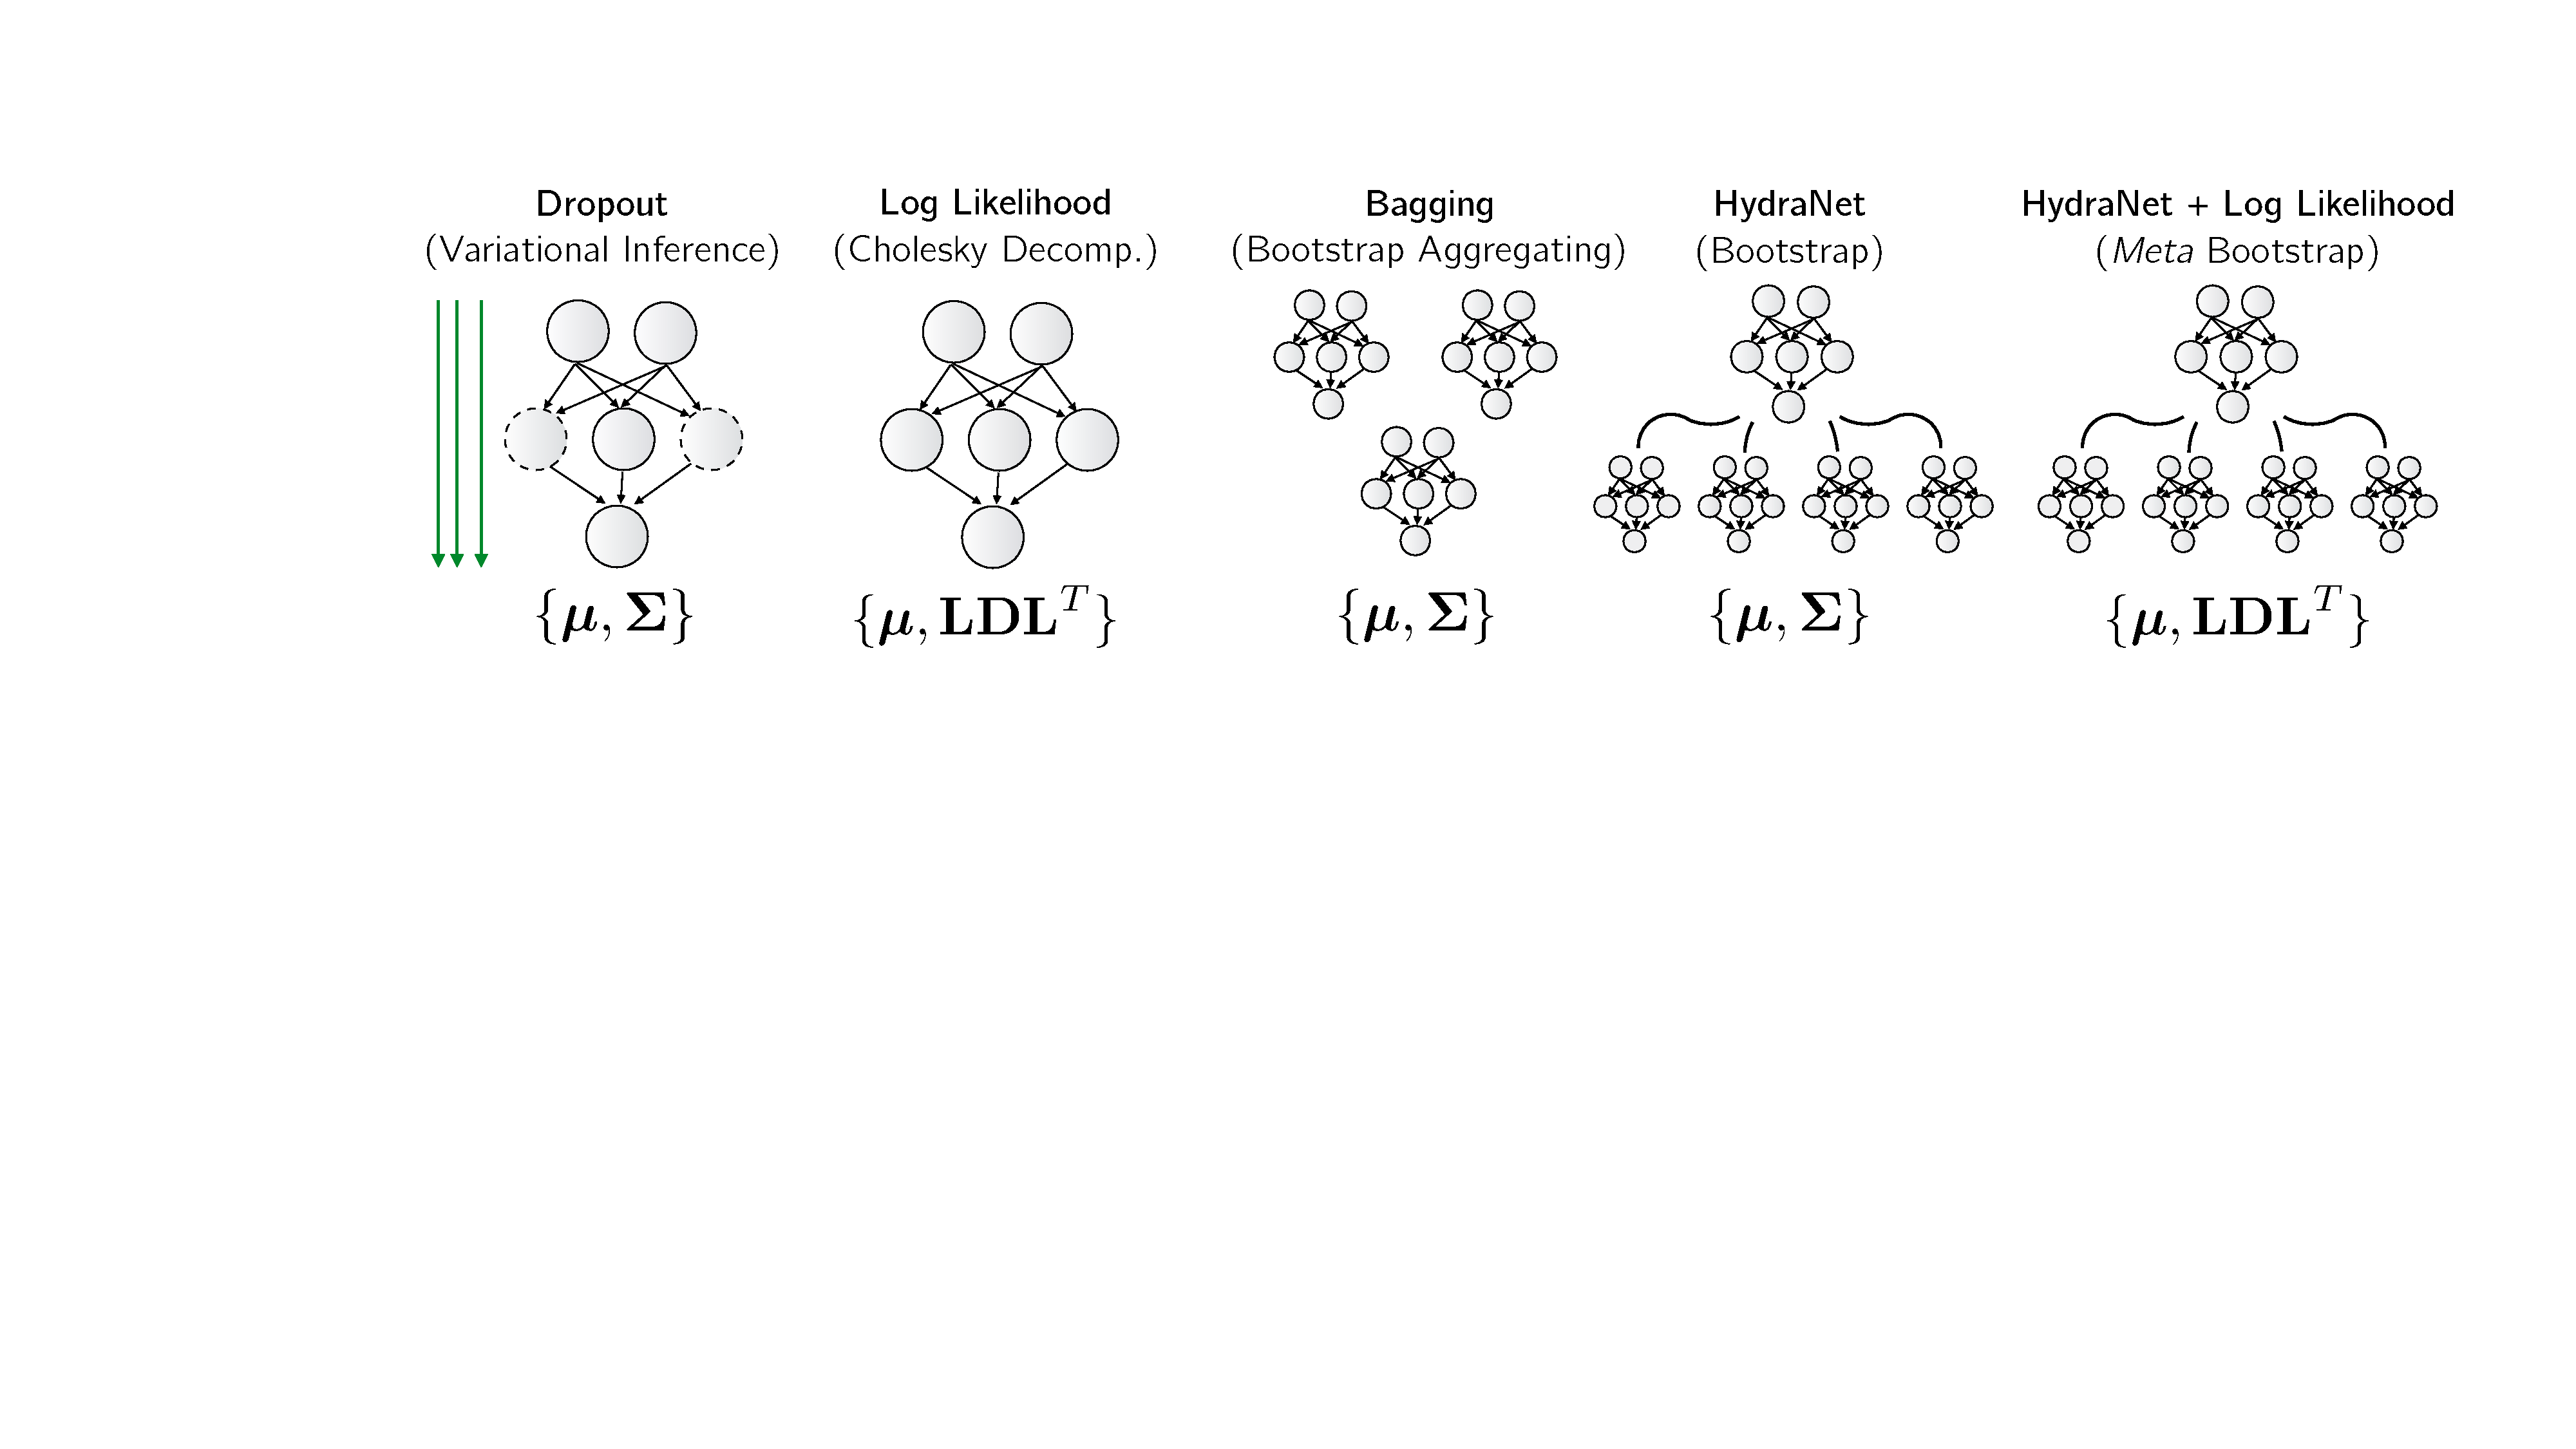
\includegraphics[width=0.95\textwidth]{lkf/nn_uncertainty.pdf}
    \caption{Different proposed uncertainty schemes for deep networks.}
    \label{fig:lkf_nn_uncertainty}    
    \end{subfigure}
    
    \begin{subfigure}[]{0.9\textwidth}
    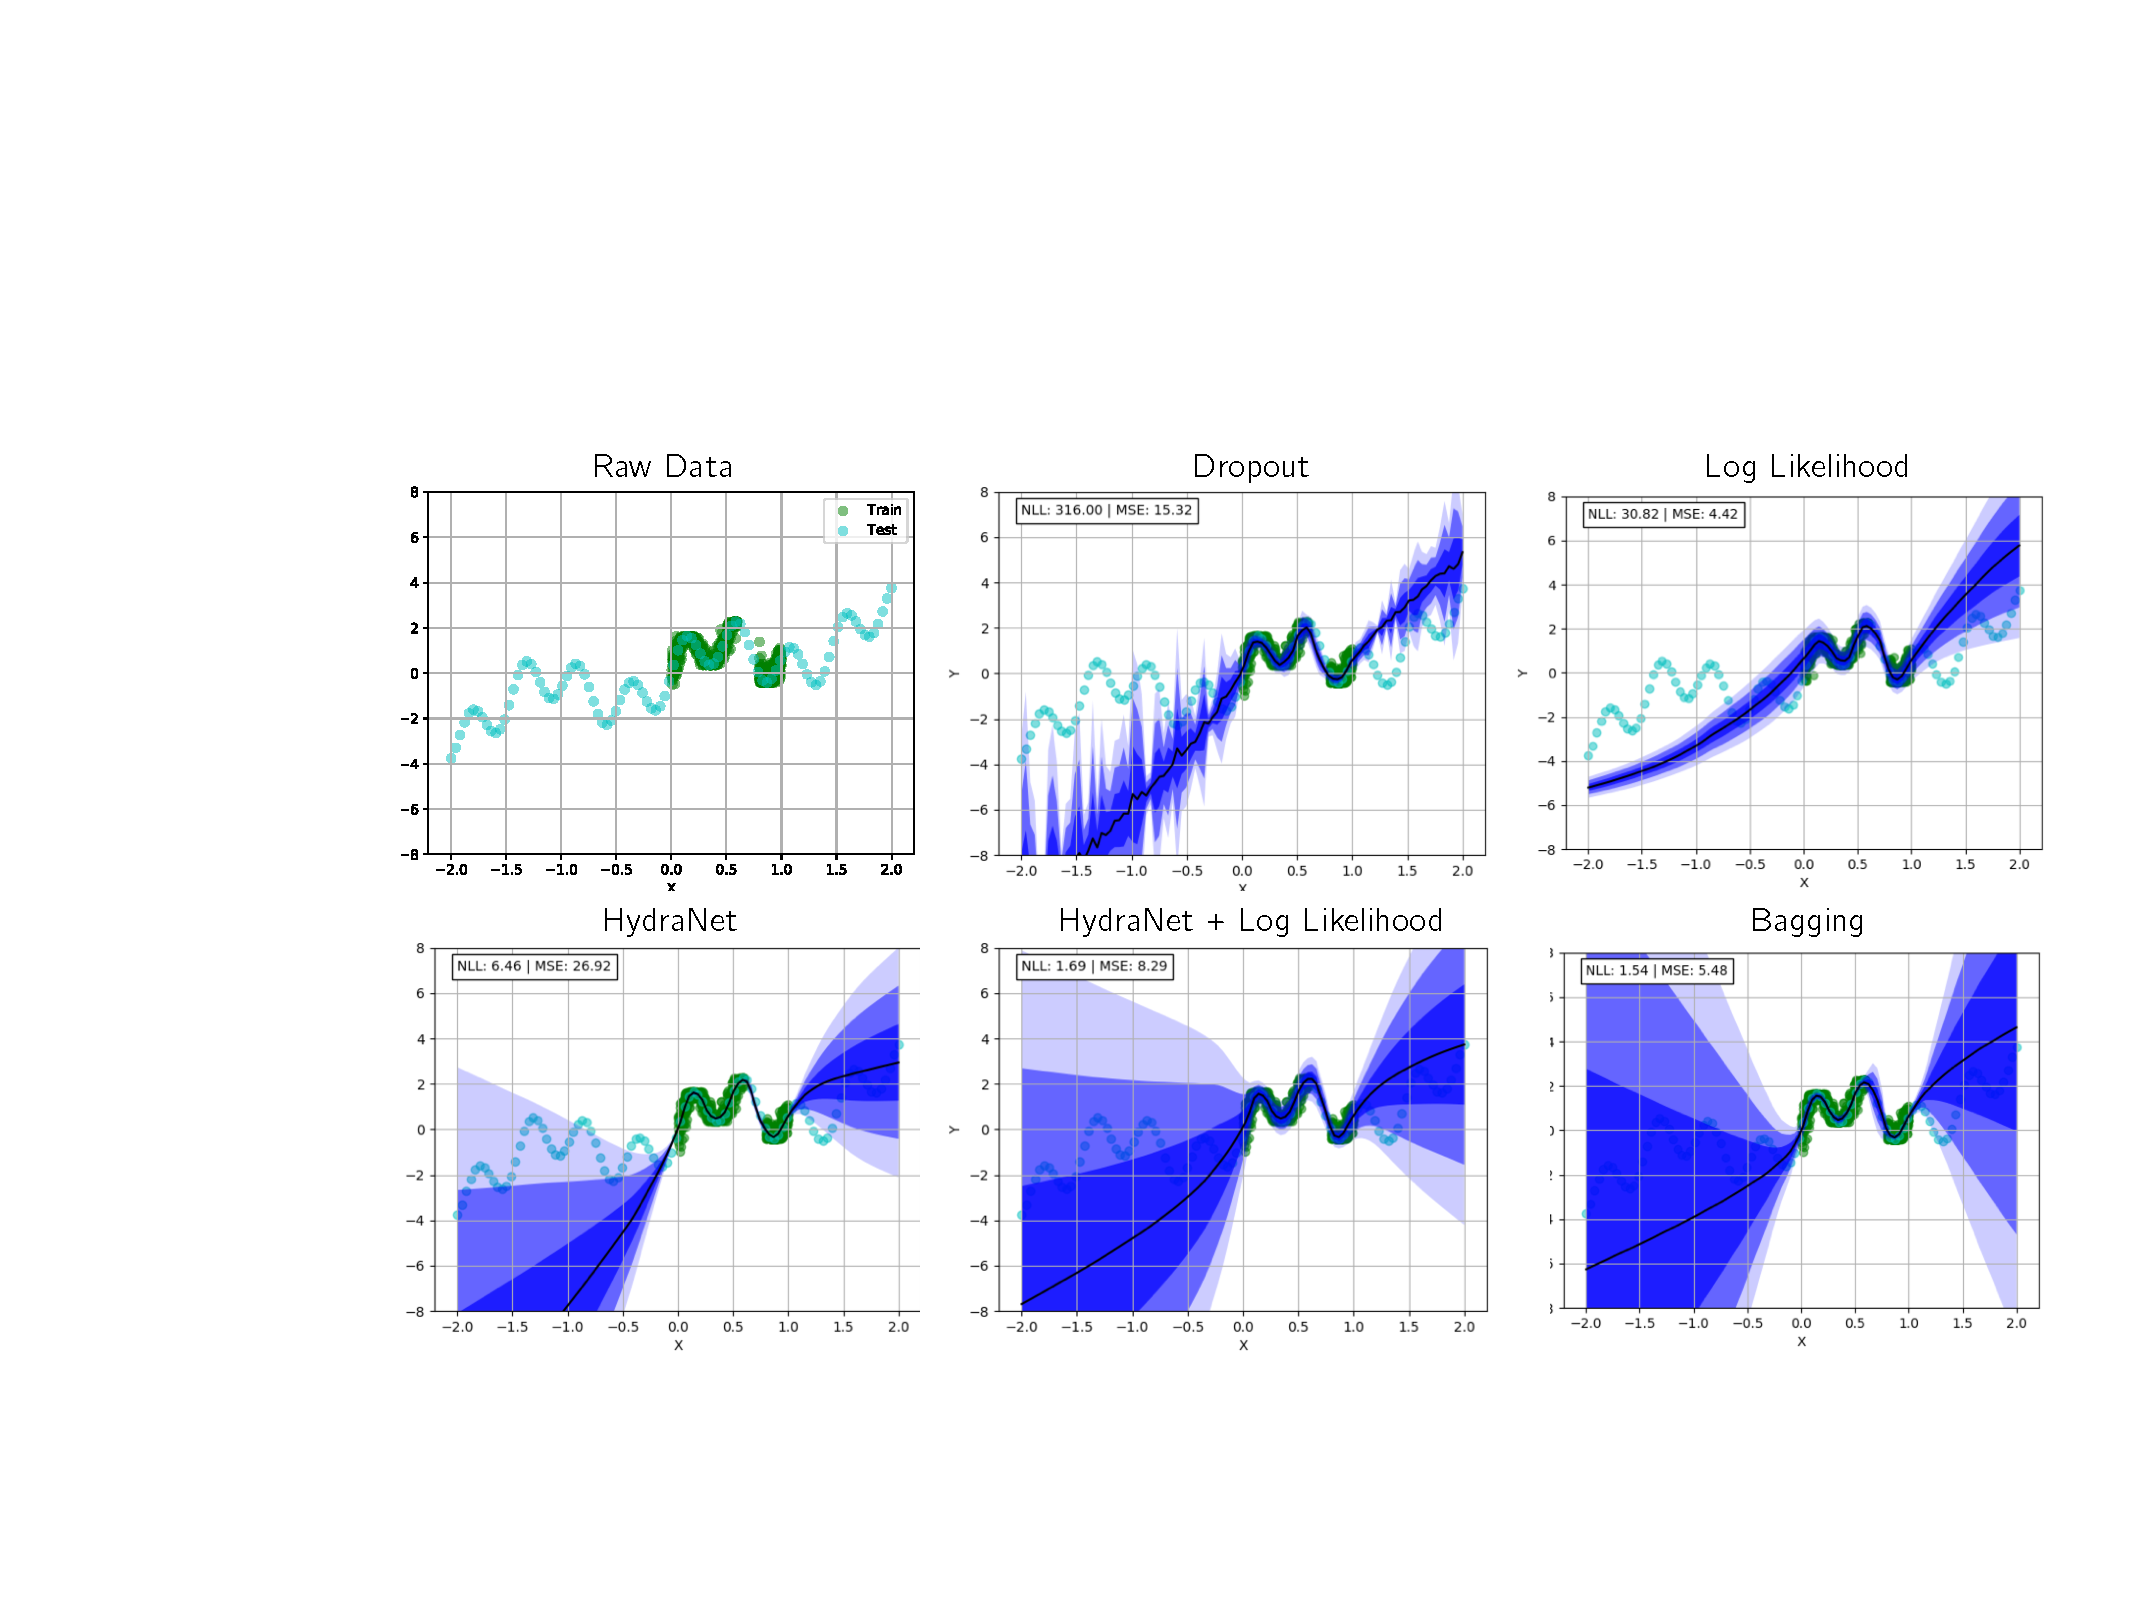
\includegraphics[width=0.95\textwidth]{lkf/uncertainty_comp.pdf}
    \caption{Comparisons of uncertainty predictions from five different probabilistic neural networks. Shades of blue represent multiples of $\sigma$. Training and test data come from the generating function $y = x + \sin{(\alpha x)} + \sin{(\beta x)}$.}
	\end{subfigure}
	\label{fig:lkf_deep-uncertainty}
	\caption{Investigations into uncertainty with deep neural networks. The network consists of two layers, with one dimensional inputs and outputs. Bagging uses 10 models and HydraNet uses 10 heads.}
\end{figure}

\section{System}


\begin{figure}
    \centering
    \begin{subfigure}[]{0.9\textwidth}
    \centering
    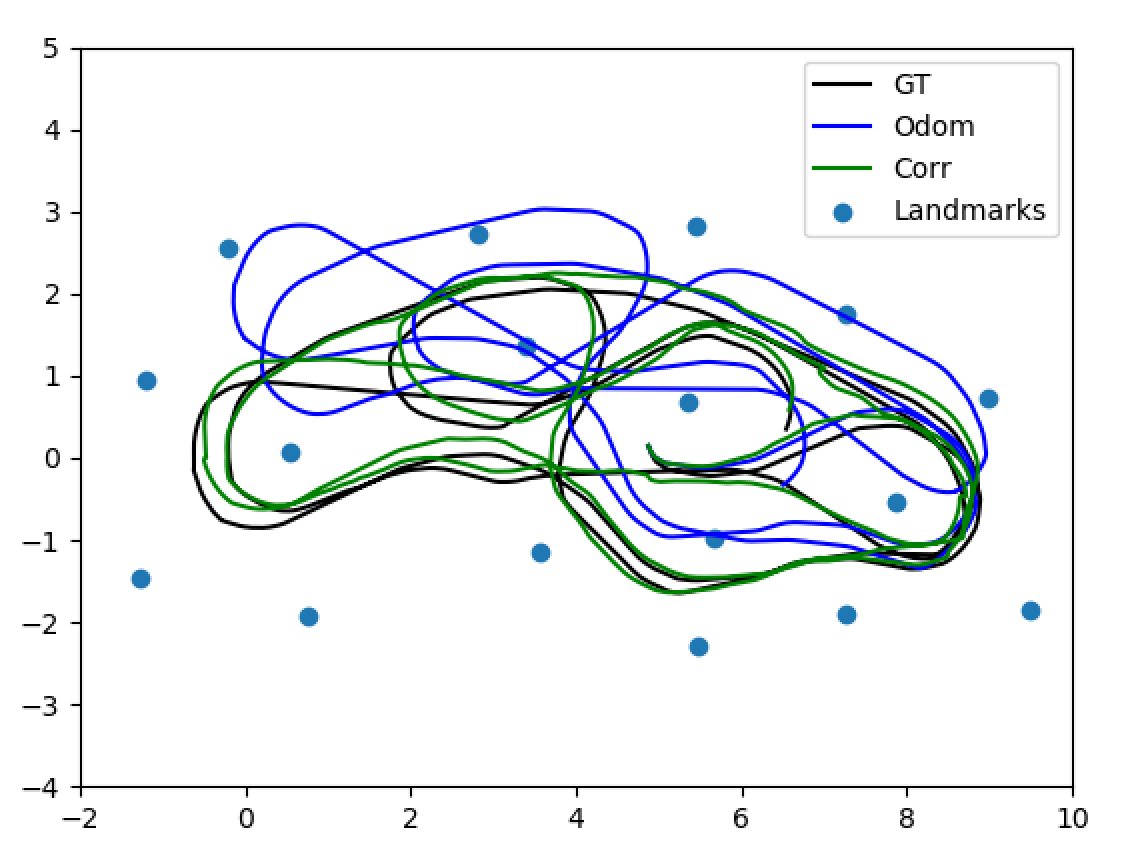
\includegraphics[width=0.75\textwidth]{lkf/a2_topdown}
	\caption{Top down view on a 2D dataset with external groundtruth every 10 seconds.}
	\label{fig:lkf_2d_topdown}    
    \end{subfigure}
    
    \begin{subfigure}[]{0.9\textwidth}
	\centering
    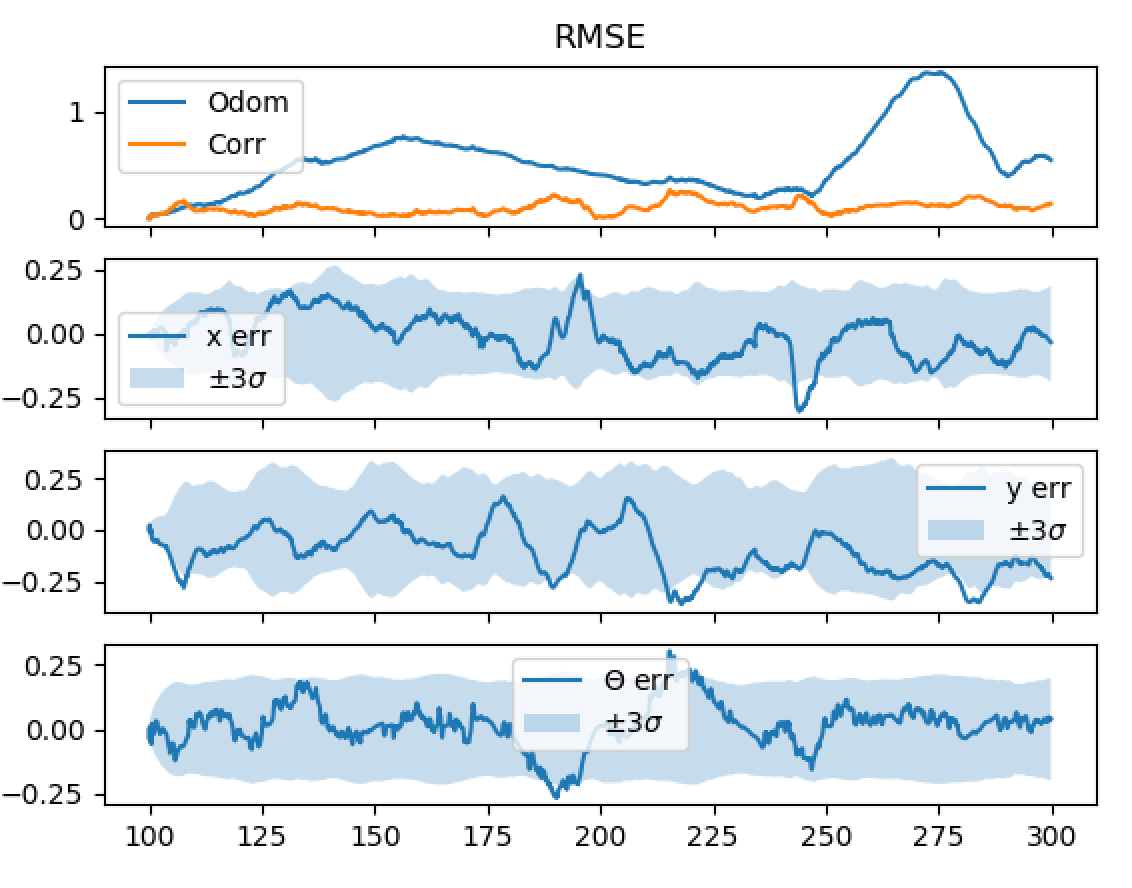
\includegraphics[width=0.75\textwidth]{lkf/a2_errors}
	\caption{Errors on a 2D dataset with external groundtruth every 10 seconds.}
	\label{fig:lkf_2d_errors} 
		\end{subfigure}
	\label{fig:lkf_2d}
	\caption{2D investigations.}
\end{figure}


\begin{figure}
	\centering
	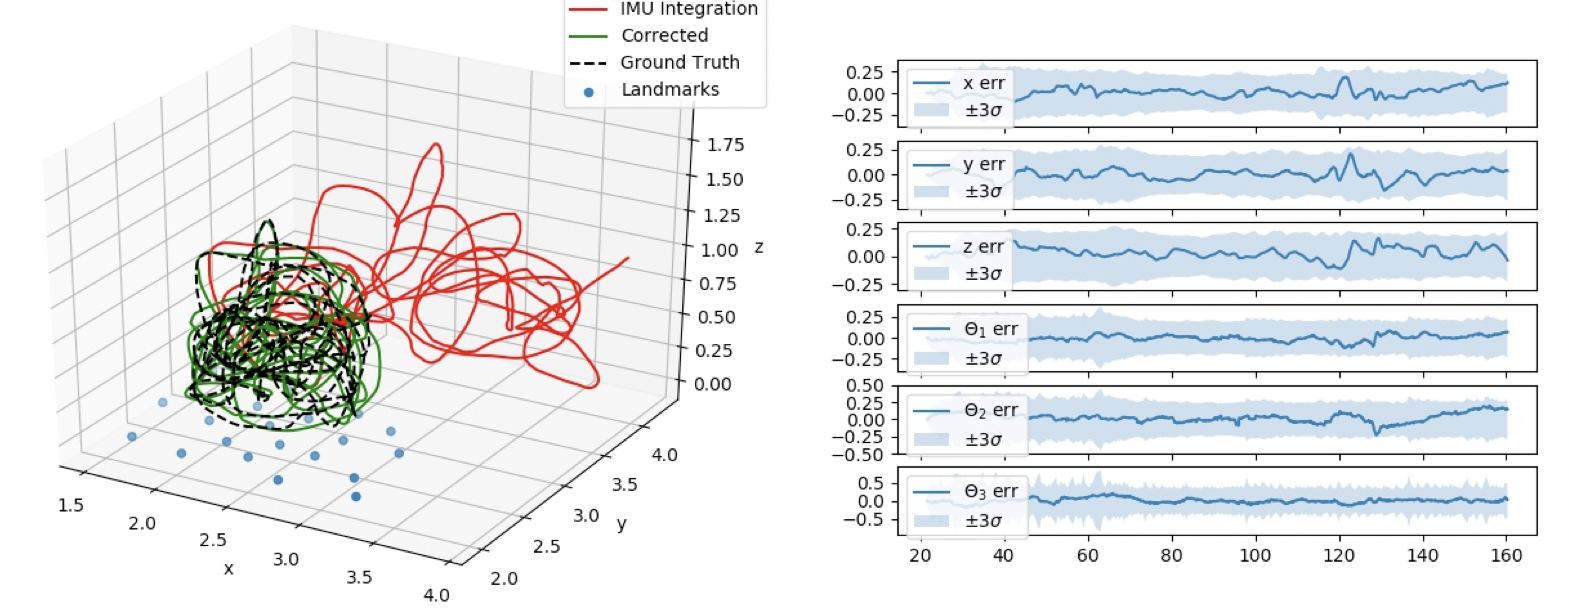
\includegraphics[width=\textwidth]{lkf/a3_combined}
	\caption{Errors on a 3D dataset with external groundtruth every 15 seconds.}
	\label{fig:lkf_system}
\end{figure}

\begin{figure}
	\centering
	\includegraphics[width=0.75\textwidth]{lkf/a3_imu-gps_combined}
	\caption{The same 3D data with a traditional Kalman filter with the same ground truth.}
	\label{fig:lkf_system}
\end{figure}



 